\section{Learning to Optimize}
To be able to learn the Q function, we need two pieces: featurized representation for the arguments ($G$ and $c$) and a way of collecting training data.

\subsection{Featurizing the Join Decision}
We need to featurize the query graph $G$ and a particular contraction $c$, which is a tuple of two vertices from the graph. 

\vspace{0.5em} \noindent \textbf{Participating Relations: } The first step is to construct a set of features to represent which relations are participating the in the query and in the particular contraction. Let $A$ be the set of all attributes in the database (e.g., $ \{Emp.id, Pos.rank,...,Sal.code,Sal.amount\}$). Each relation $r$ (including intermediate relations that are the result of join) has a set of \emph{visible attributes}; those attributes present in the output $A_r \subseteq A$. So every query graph $G$ can be represented by its visible attributes $A_G$. Each contraction is a tuple of two relations $(l,r)$ and we can get the visible attributes $A_l$ and $A_r$ for each. Each of these subsets $A_G, A_l, A_r$ can be represented with a binary 1-hot encoding representing which subset of the attributes are present. We call the concatenation of these vectors $V_{rel}$ and it has dimensionality of $3\cdot|A|$. Figure \ref{feat} illustrates the featurization on the example query in the background section. 

\begin{figure*}
    \centering
    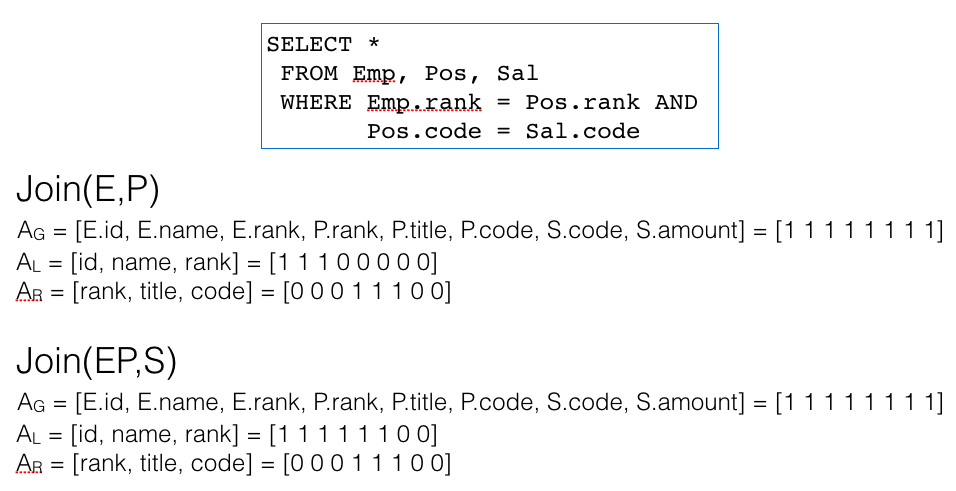
\includegraphics[width=0.7\textwidth]{figs/featurization.png}
    \caption{We use 1-hot encoding to capture which attributes participate in a join. This allows us to featurize both the query graph and the contraction. This figure shows the featurization for two different joins for the example query. \label{feat}}
\end{figure*}

To handle single relation selections in the query, we have to tweak the feature representation. This is because upstream selections and projections will change the cost properties of downstream joins. As in the classical optimizers, we eagerly apply selections and projections to each relation. 
Here, we leverage the table statistics present in most RDBMS. For each relation in the query graph, we can estimate a reduction factor $\delta_{r}$, which is an estimate of the fraction of tuples present after applying the selection to relation $r$. 
In the featurization described in the previous section, we have a set of binary features $V_{rel}$ that describe the participating attributes.
We multiply the reduction factors $\delta_r$ for each table with the features corresponding to attributes derived from that relation.
Figure \ref{feat:sel} illustrates the effect of adding a single table predicate to the example query. 

\begin{figure}
    \centering
    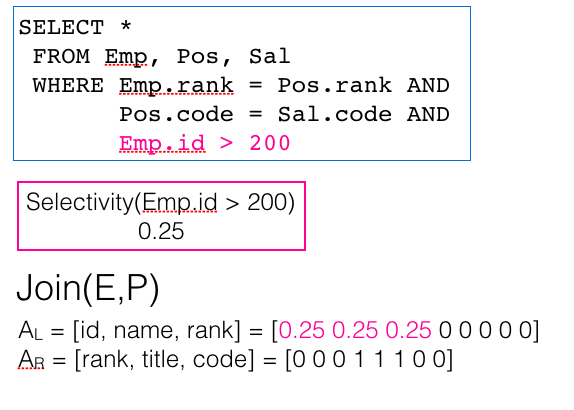
\includegraphics[width=\columnwidth]{figs/selectivity.png}
    \caption{To featurize single table selections, we scale the features by selectivity estimates given to use from a cost-estimator. \label{feat:sel}}
\end{figure}

\vspace{0.5em} \noindent \textbf{Join Condition: } The next piece is to featurize the join condition, or the predicate that defines the join. Participating relations define vertices and the predicate defines an edge. As before, let $A$ be the set of all attributes in the database. Each expression has two attributes and an operator. As with featurizing the vertices we can 1-hot encode the attributes present. We additionally have to 1-hot encode the binary operator $\{=,!=,<,>\}$. Concatenating all of these binary vectors together for each expression $\rho$ there there is a binary feature vector $f_\rho$.  For each of the expressions in the conjunctive predicate, we concatenate the binary feature vectors. Here is where the fixed size assumption is used. Since the maximum number of expressions in the conjunction capped at $\mathcal{N}$, we can get a fixed sized feature vector for all predicates. We call this feature vector $V_{cond}$ and it has dimensionality of $\mathcal{N} \cdot(|A|+4)$. 

\vspace{0.5em} \noindent \textbf{Representing the Q-Function: }
The Q-function is represented as a multi-layer perceptron (MLP) neural network.
It takes as input two feature vectors $V_{rel}$ and $V_{cond}$. Experimentally, we found that a two-layer MLP gave the best performance relative to the training time. We implmented the training algorithm in \textsf{DL4J} a java framework for model training with a standard DQN algorithm. The featurization approach is very extensible. Any property that we want the network to capture and be robust to can be added to the feature representation. For example, we can add an addition set of binary features $V_{ind}$ that indicate which attributes have indexes built on them. Handling, sort-orders are similar and we have to add features describing which attributes need to be finally sorted in the query. We can similarly add features that describe the available memory if we believe that is an important resource to manage in determining the final best plan.

\vspace{0.5em} \indent \textbf{Training: }

\[
\theta^{(i+1)} = \theta^{(i)} + \alpha \cdot [ (R + \max_{c'} Q_\theta(G',c')) - Q_\theta(G,c) ] \cdot \nabla Q_\theta(G,c) 
\]

\subsection{Generating the Training Data}
Experimentally, we found that the process of generating the process of training data for a given workload was very important for robust learning.
The basic challenge is that the Q-function must accurately be able to differentiate between good plans and bad plans.
If the training data only consisted of optimal plans, then the learned Q-function may not accurately score poor plans. Likewise, if the training purely sampled random plans--it may not see very many instances of good plans.
We want an efficient algorithm that avoids exhaustive enumeration to sample a variety of very good plans and poor plans.

The data generation algorithm, which we denote as \textsf{sample}$(G, \epsilon)$, takes as input a query graph $G$ and a randomization parameter $\epsilon \in [0,1]$.

\textsf{sample}$(G, \epsilon)$:
\begin{enumerate}
    \item \textbf{if} $\kappa_G = |G|$ return.
    \item For all graph contractions $c_i$ on G:.
    \begin{enumerate}
    \item $G_i = c_i(G)$  
    \item $V(c_i, G_i) = \textsf{leftDeep}(G_i)$
    \end{enumerate}
    \item \textbf{if} \textsf{rand()} $> \epsilon$: yield $c_j, G_j = \arg\max_{c_i} V(c_i,G_i)$, return \textsf{sample}$(G_j,\epsilon)$
    \item \textbf{else: } yield uniform random $c_j, G_j $, return \textsf{sample}$(G_j,\epsilon)$
\end{enumerate}

The algorithm essentially acts as the Q-Function algorithm described in the previous section. The algorithm proceeds as follows: (1) start with the query graph, (2) find the lowest cost contraction, (3) update the query graph and repeat. The lowest cost contraction is determined by assuming the remaining joins will be optimized with a left-deep strategy.
Let \textsf{leftDeep}(G) be the function that calculates the final cost of the best left deep plan given the query graph G.
To implement \textsf{leftDeep}(G), we use the System R dynamic program. 
This acts as an approximation to the Q function where the current step is locally optimal but future joins are efficiently approximate. {\reminder {Zongheng: I don't understand what ``efficiently approximate'' means. Do you mean ``efficiently approximated''?}}

To sample some number of poor plans in the training dataset, the $\epsilon$ parameter controls the number of randomly selected decisions.
This trades off reasonable optimality during training vs. covering the space of plans.
In this sense, we base the data generation algorithm in a particular \emph{workload}. The workload is a distribution over join queries that we want to optimize. 
We have an optimizer that samples some number of initial queries from the workload and is tested on unseen data.

\subsection{Execution after Training}
After training, we will have a parametrized estimate of the Q-function, $Q_\theta(f_G,f_c)$. For execution, we simply go back to the standard algorithm as in the greedy method but instead of using the local costs, we use the learned Q-function: (1) start with the query graph, (2) featurize each contraction (2) find the contraction with the lowest \textbf{estimated Q-value}, (3) update the query graph and repeat.
